\documentclass[a4paper,utf8]{article}
\usepackage[heading,fancyhdr]{ctex}
\usepackage{amsmath,amssymb,geometry,lastpage,ulem}
\usepackage{array,tabularx,tabulary,mhchem,xspace}
\usepackage{floatrow,subfig,multirow,bigstrut}
\usepackage{siunitx,booktabs,longtable,graphicx,xfrac,nameref}
\lineskiplimit=1pt
\lineskip=3pt
\geometry{
    top=25.4mm, 
    left=25mm, 
    right=25mm, 
    bottom=25mm,
    headsep=5.9mm,
}
\ctexset{
    section = {format+=\raggedright}
}
\newcommand{\fgref}[1]{图~\ref{#1}\xspace}
\newcommand{\seqref}[1]{式~(\ref{#1})}
\newcommand{\expinfo}[7][无]{
    {\zihao{-3}\bfseries\songti
    实验名称:\uline{\hfill\mbox{#2}\hfill} \\[2.9mm]
    学\quad 号:\uline{\makebox[25mm]{#3}}\hfill
    姓\quad 名:\uline{\makebox[25mm]{#4}}\hfill
    班\quad 级:\uline{\makebox[25mm]{#5}} \\[2.9mm]
    合作者:\uline{\makebox[25mm]{#1}} \hfill
    桌\quad 号:\uline{\makebox[25mm]{#6}}\hfill\makebox[25mm+4em]{}\\[2.9mm]
    实验日期:\uline{\makebox[30mm]{#7}}\hfill\mbox{} \\[58.7mm]
    }
}
\newcommand{\pointingbox}{
    {\zihao{4}\bfseries\songti%
    实验考核\\[3mm]
    \extrarowheight=3mm
    \begin{tabularx}{150mm}{|X|X|X|X|X|}\hline
        \hfil 项目 \hfil  & \hfil 实验预习 \hfil & \hfil 实验过程 \hfil & \hfil 分析与讨论 \hfil & \hfil 总评 \hfil \\[3mm] \hline
        \hfil 评价 \hfil &  &  &  &  \\[3mm] \hline
    \end{tabularx}
    }
}
\newcommand{\derivative}[2]{\frac{\mathrm{d} #1}{\mathrm{d} #2}}
\newcommand{\thinking}[2]{\textbf{#1}\\
答:\begin{minipage}[t]{0.85\textwidth}
    #2
\end{minipage}}
\pagestyle{fancy}
\fancyhf{} \fancyhead[C]{电路基础实验} \fancyfoot[C]{\thepage~/~\pageref{LastPage}}
\newcounter{Rownumber}
\newcommand*{\Rown}{\stepcounter{Rownumber}\theRownumber}
\newcommand*{\resetRown}{\setcounter{Rownumber}{0}}
\newcommand{\qrange}[3]{\qtyrange[range-phrase = \text{$\sim$},range-units =single]{#1}{#2}{#3}}
\floatsetup[table]{capposition=top}
\newcolumntype{C}{>{\hfil}X<{\hfil}}
\renewcommand{\Nameref}[1]{\textbf{\ref{#1}~\nameref{#1}}} %导入导言

\begin{document}
\begin{center}
    {\mbox{}\\[7em]\zihao{2}\bfseries\songti%
    电路基础实验报告}\\[34mm]
    \expinfo[张泽钒]{R、L、C 元件阻抗特性的研究}{22301077}{张蕴东}{22 高分子}{35}{2024.6.18}
\end{center}
\newpage

\section{实验目的}
    \begin{enumerate}
        \item 验证电阻、感抗、容抗与频率的关系,测定 $R-f$、$X_\text{L}-f$ 及 $X_\text{C}-f$ 特性曲线。
        \item 加深理解 R、L、C 元件端电压与电流间的相位关系。
    \end{enumerate}

\section{实验原理}%简单描述,含必要的公式和附图;
    在正弦交变信号作用下,$R$、$L$、$C$ 电路元件在电路中的抗流作用与信号的频率有关。\par
    改变信号源频率,测量 $R$、$L$、$C$ 元件两端电压 $U_\text{R}$、$U_\text{L}$、$U_\text{C}$,流过被测元件的电流则可由 $r$ 两端电压除以 $r$ 得到。\par
    元件的阻抗角(即相位差 $\varphi$)随输入信号的频率变化而改变,将各个不同频率下的相位差画在以频率 f 为横坐标、阻抗角 $\varphi$ 为纵座标的座标纸上,并用光滑的曲线连接这些点,即得到阻抗角的频率特性曲线。 

\section{实验仪表}
    实验电路见电路原理实验箱《R、L、C 元件阻抗特性的研究》单元,$L=\SI{10}{\mH}$,$r=\SI{1000}{\ohm}$,$C=\SI{1}{\uF}$。

\section{实验内容}
    \begin{enumerate}
        \item 测量 $R$、$L$、$C$ 元件的阻抗频率特性。
        \item 用双踪示波器观察 RL 串联和 RC 串联电路在不同频率下阻抗角的变化情况。
    \end{enumerate}

\section{实验结果与分析}
    \subsection{实验数据}
        相较于使用数格子的方法,我们采用了更精确的数据采集方案。使用示波器采集的周期替代 $n$ ,再用示波器采集的相位差(或使用光标追踪)替代 $m$ ,全程完全不涉及估读等损失精度的操作。具体数据见附页,下面着重展示数据处理结果。
    \subsection{数据分析处理}
        \begin{align*}
            \left|Z\right|&=\sqrt{R^2+X^2} & X_\text{L} &= \mathrm{j} \omega L=\mathrm{j} 2\pi f L\\\
            \varphi&=\arctan\left(\frac X R\right) & X_\text{C} &= \frac{1}{\mathrm{j} \omega C}=\frac{1}{\mathrm{j} 2\pi f C}
        \end{align*}
        电阻的$R-f$关系为一条平行 x轴的直线,$R_\text{Measure}=999.41\unit{\ohm}$,从原理上讲其不随输入频率变化而变化,但测量时会因为频率上升至接近采样率上限而失真,故不展示图。\newpage
        电感和电容的阻抗是会随着频率变化而改变的,这是因为其实部电阻部分不变但虚部电抗部分是一个与频率相关的值,因此模会发生改变。考虑到测量的对象并非理想电感器和理想电容器,根据上面的公式可以拟合出的结果如下图:\par
        \begin{figure}[!ht]
            \subfloat[$Z_\text{L}-f$]{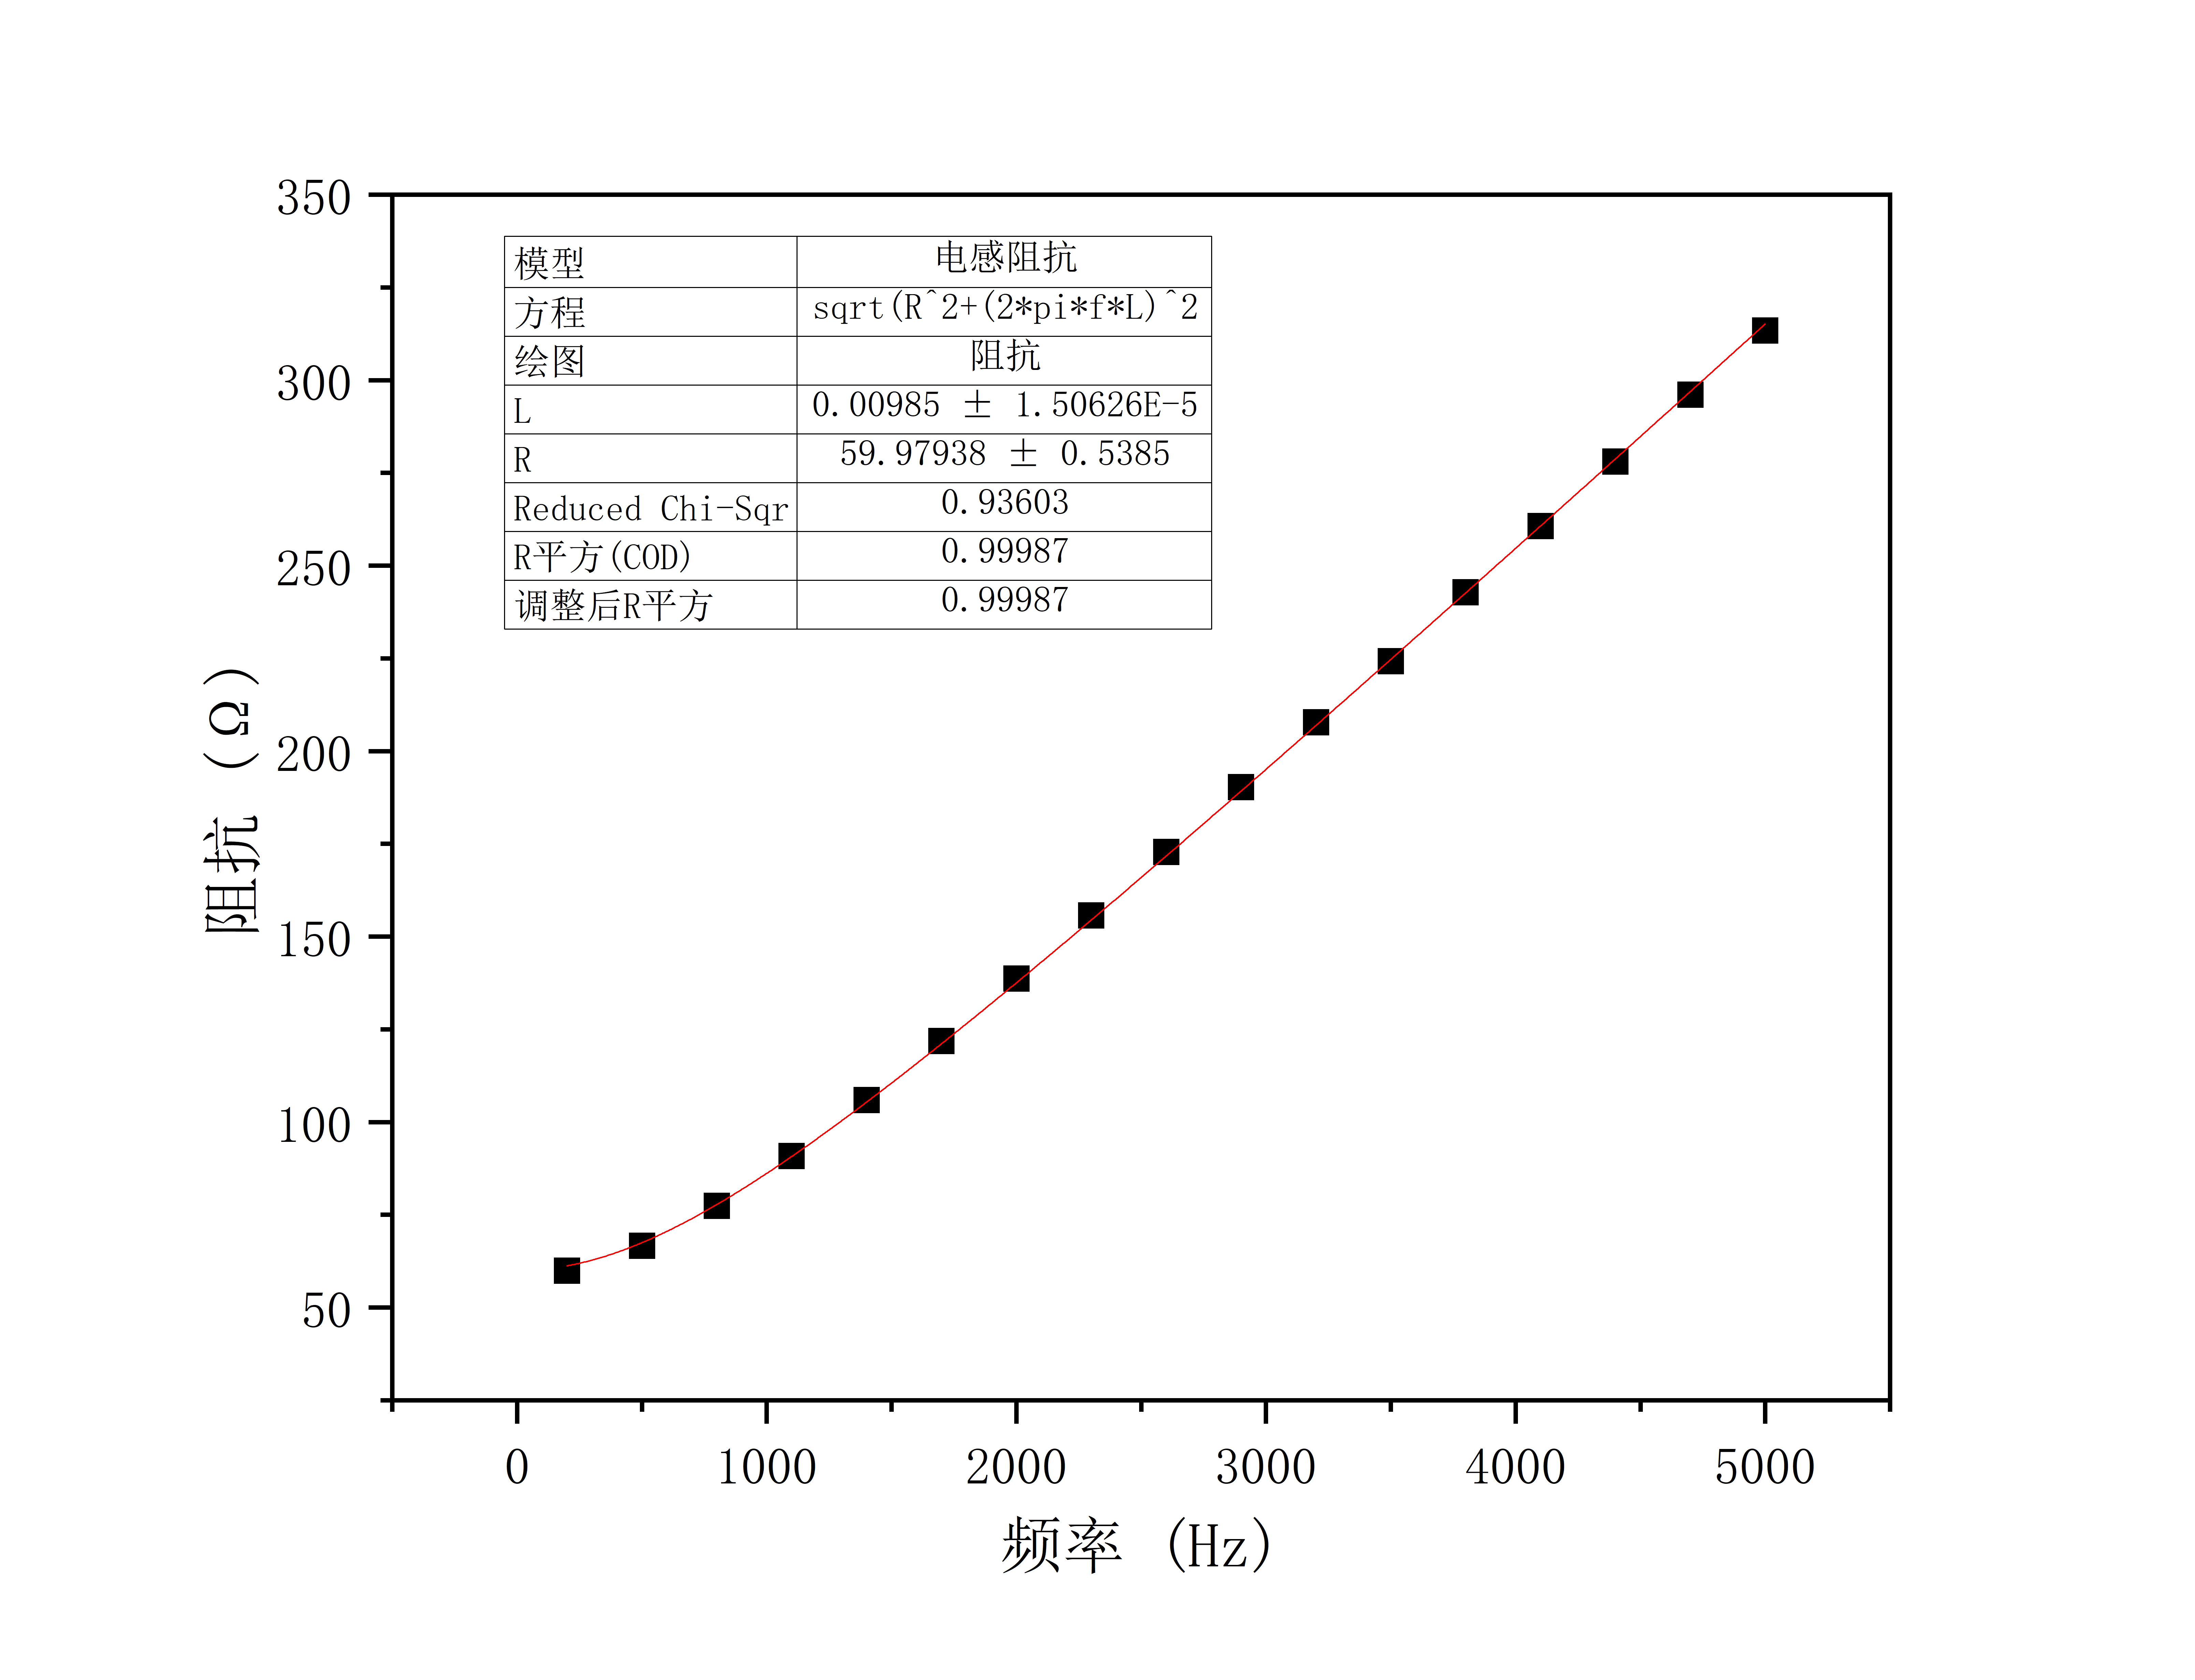
\includegraphics[width=0.7\textwidth]{1.png}}\\
            \subfloat[$Z_\text{C}-f$]{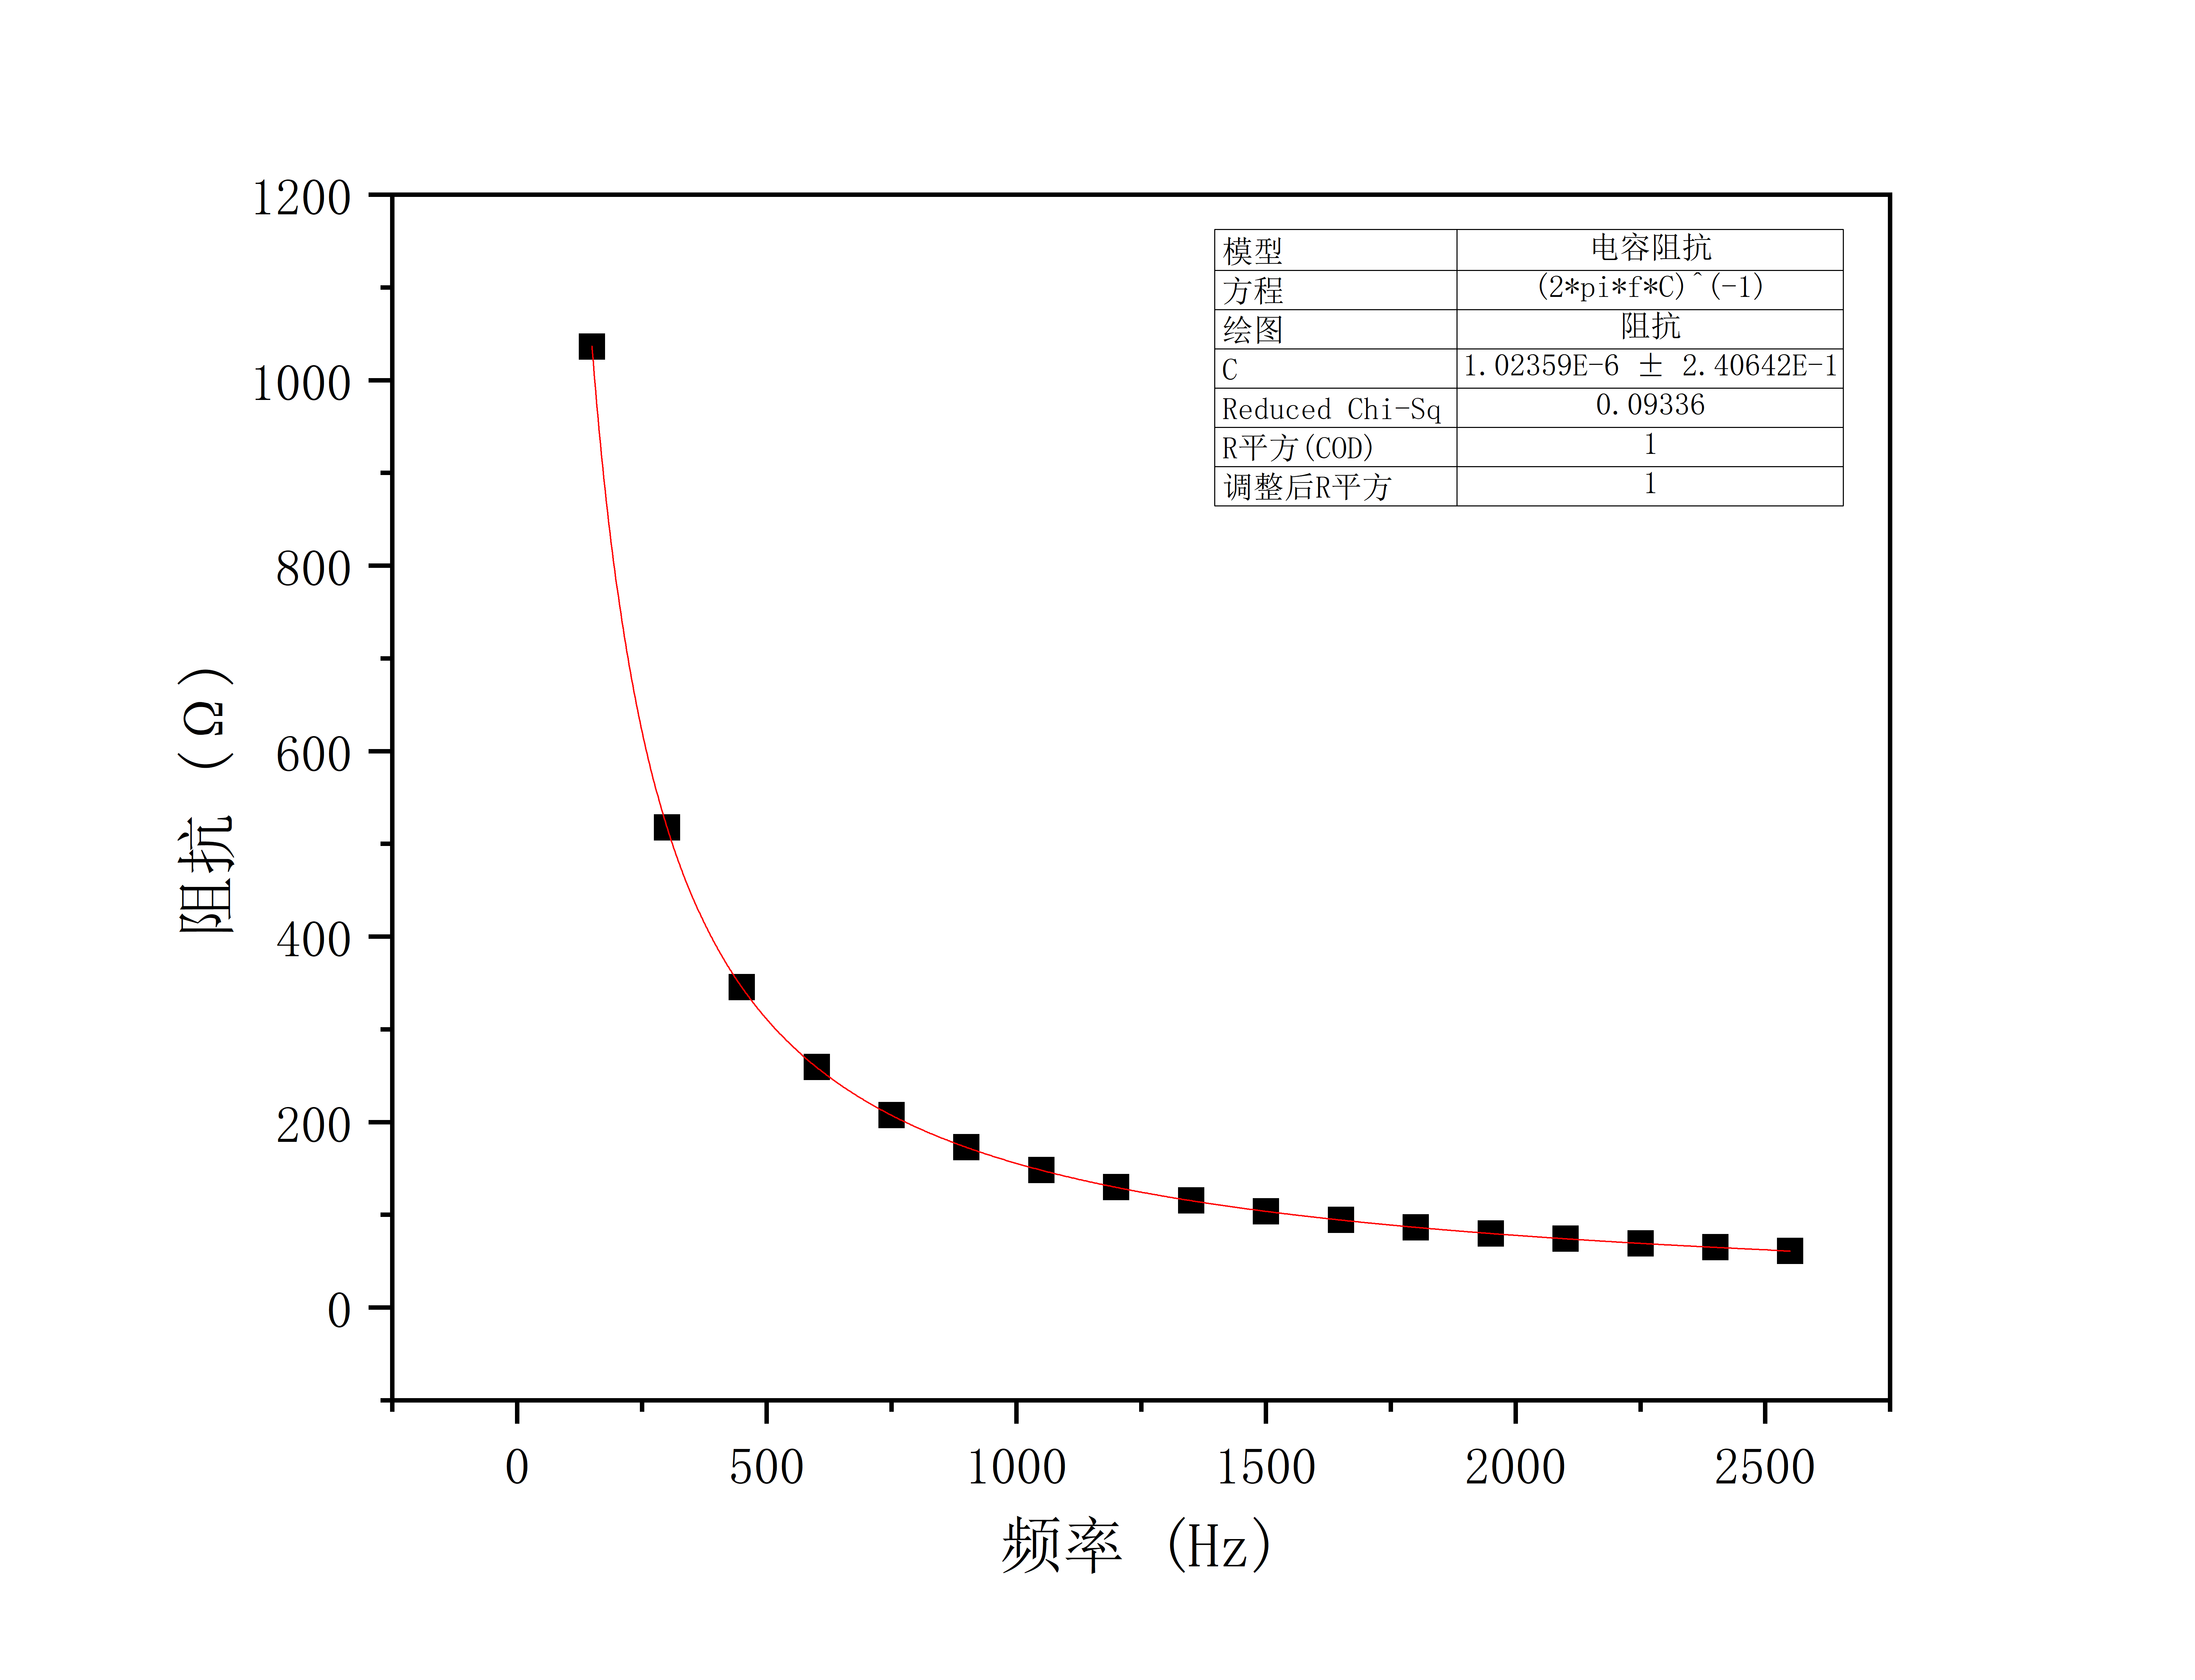
\includegraphics[width=0.7\textwidth]{2.png}}\\
            \caption{阻抗与频率关系曲线\label{fig:1}}
        \end{figure}\par
        \newpage
        由图可见,拟合出来的电感值为 $L=9.85\unit{\mH}$ ,电感本身的阻值为 $R_\text{L}=59.97\unit{\ohm}$;电容值为 $C=1.02\unit{\uF}$ ,其电阻值在实际测量中影响很小,约为 $R_\text{C}=17\unit{\ohm}$ (这里并没有专门在 Origin 中拟合出来,只在 Mathematica 中有相关计算)。拟合值与实际值的差别很小,也可以反映出本方法的精确性。\par
        接着是阻抗角与频率的关系曲线:\par
        \begin{figure}[!ht]
            \subfloat[$\varphi_\text{L}-f$]{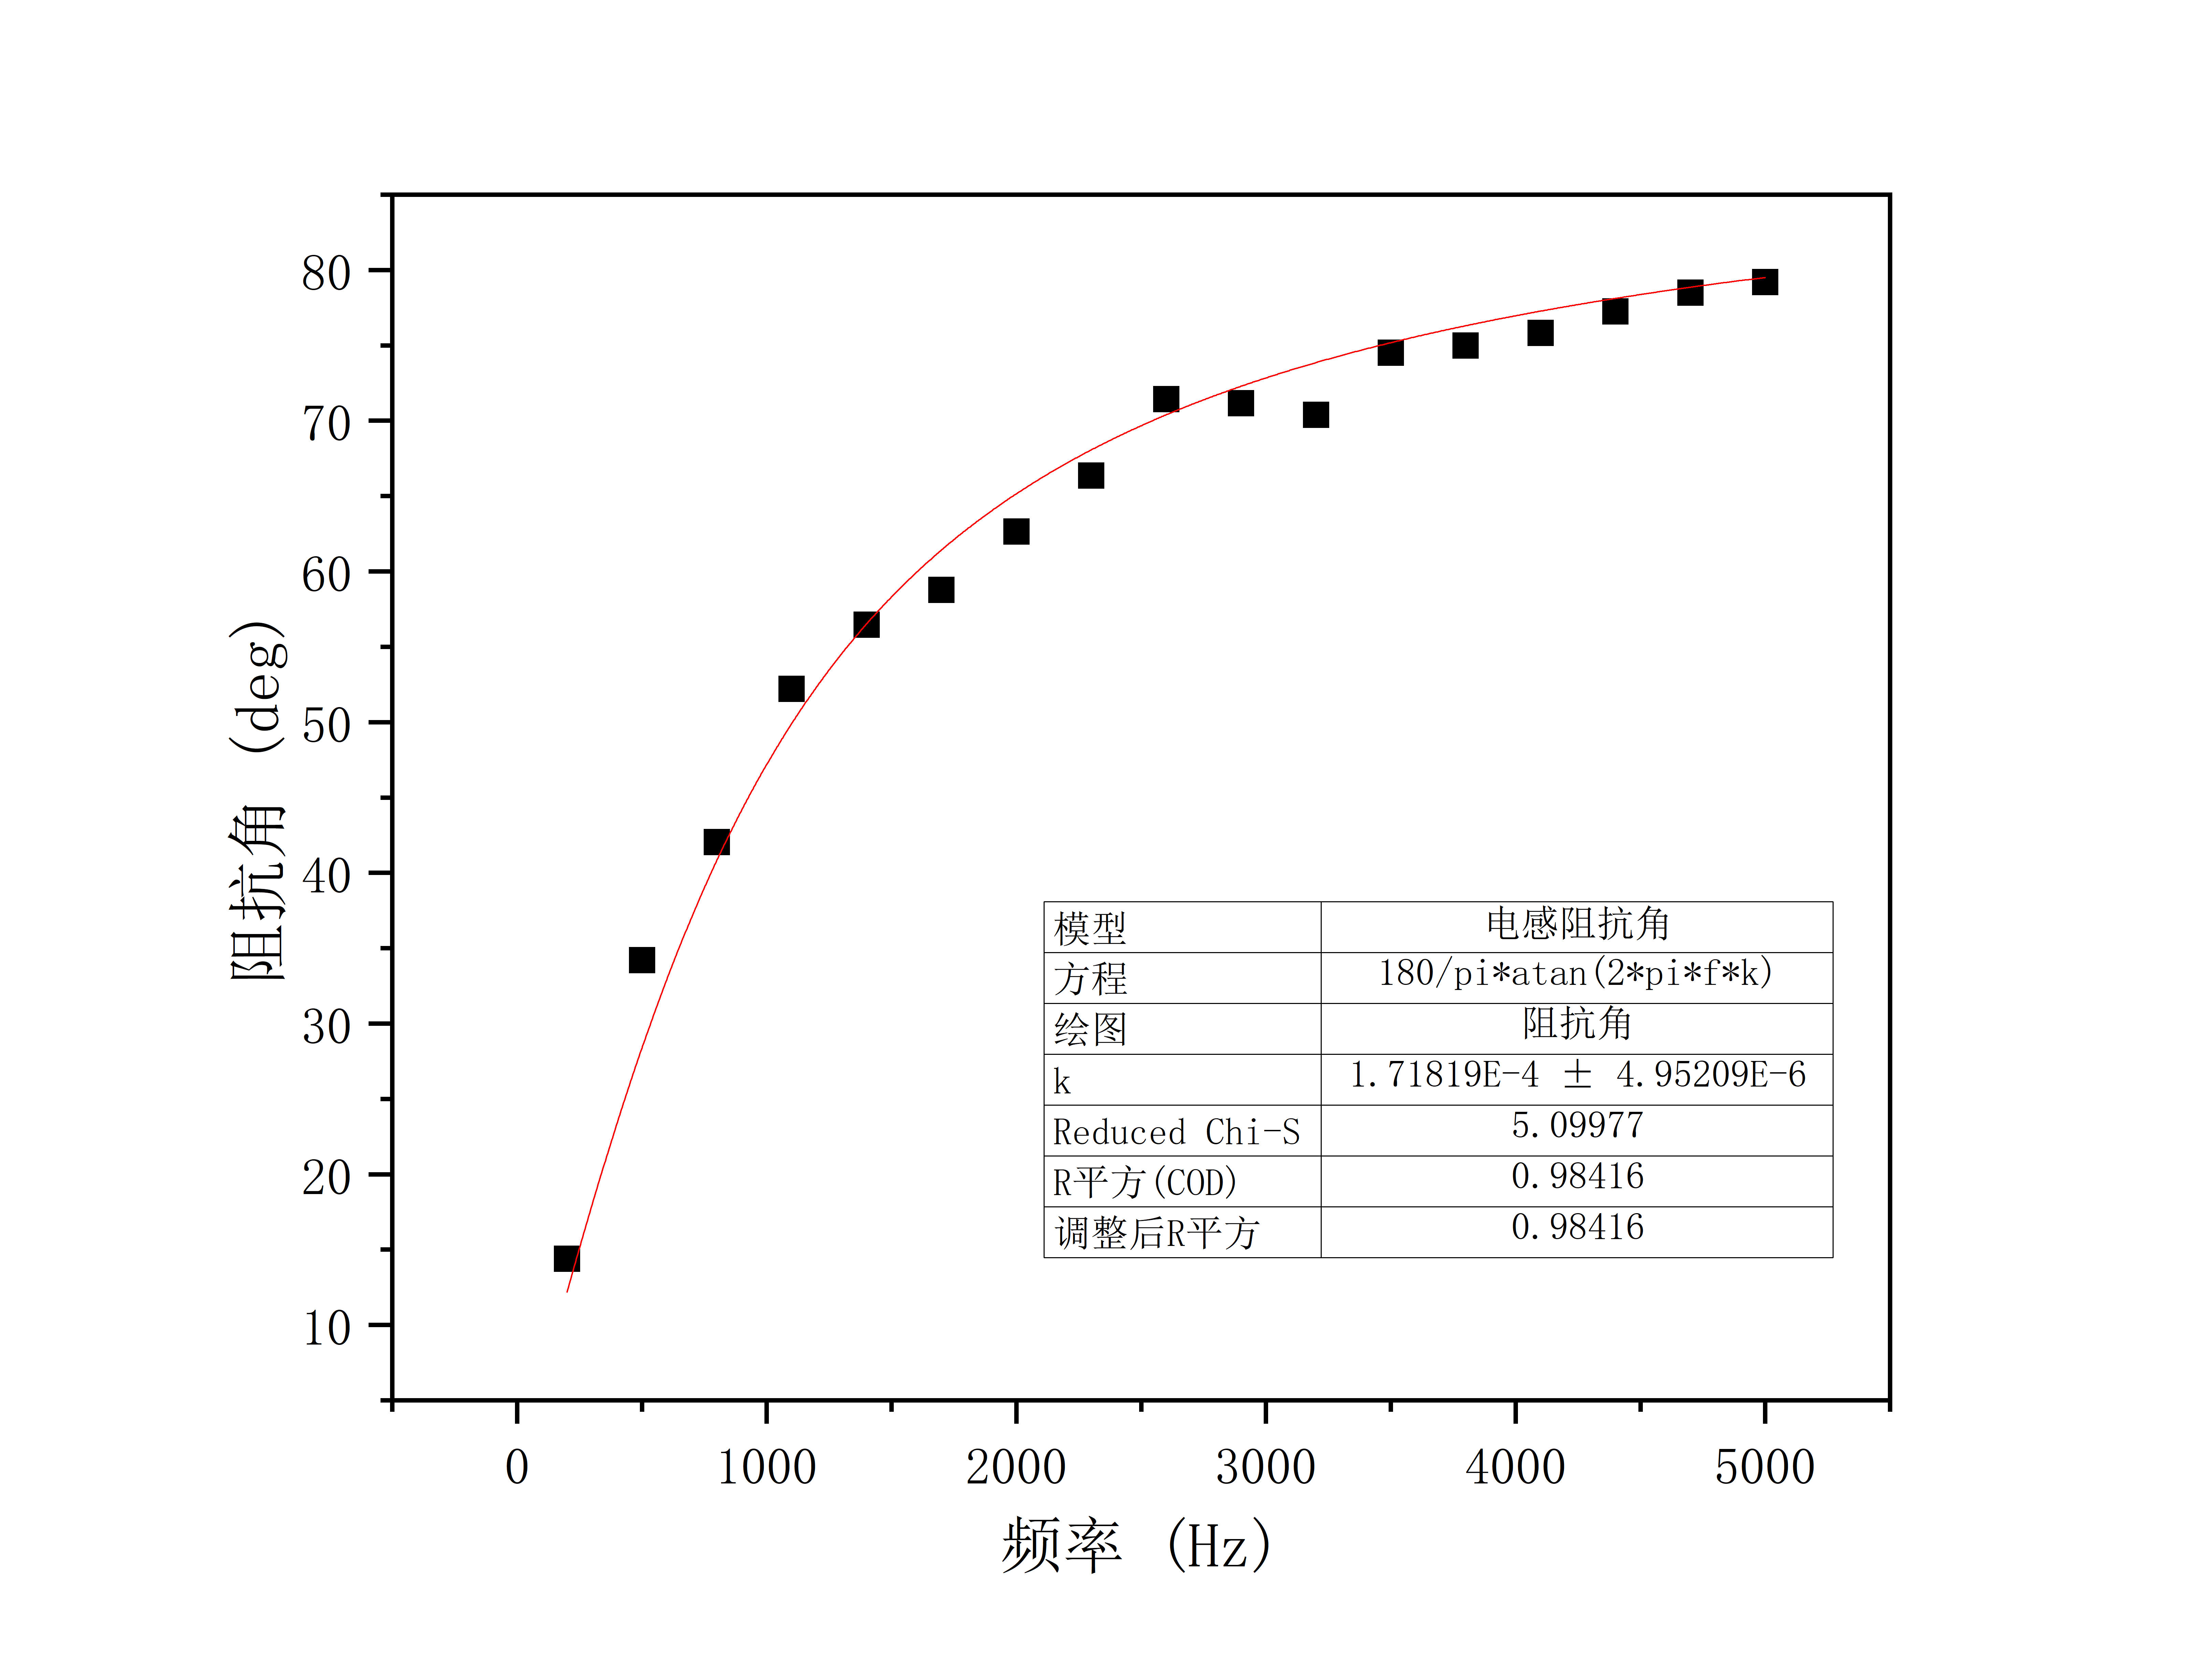
\includegraphics[width=0.7\textwidth]{3.png}}\\
            \subfloat[$\varphi_\text{C}-f$]{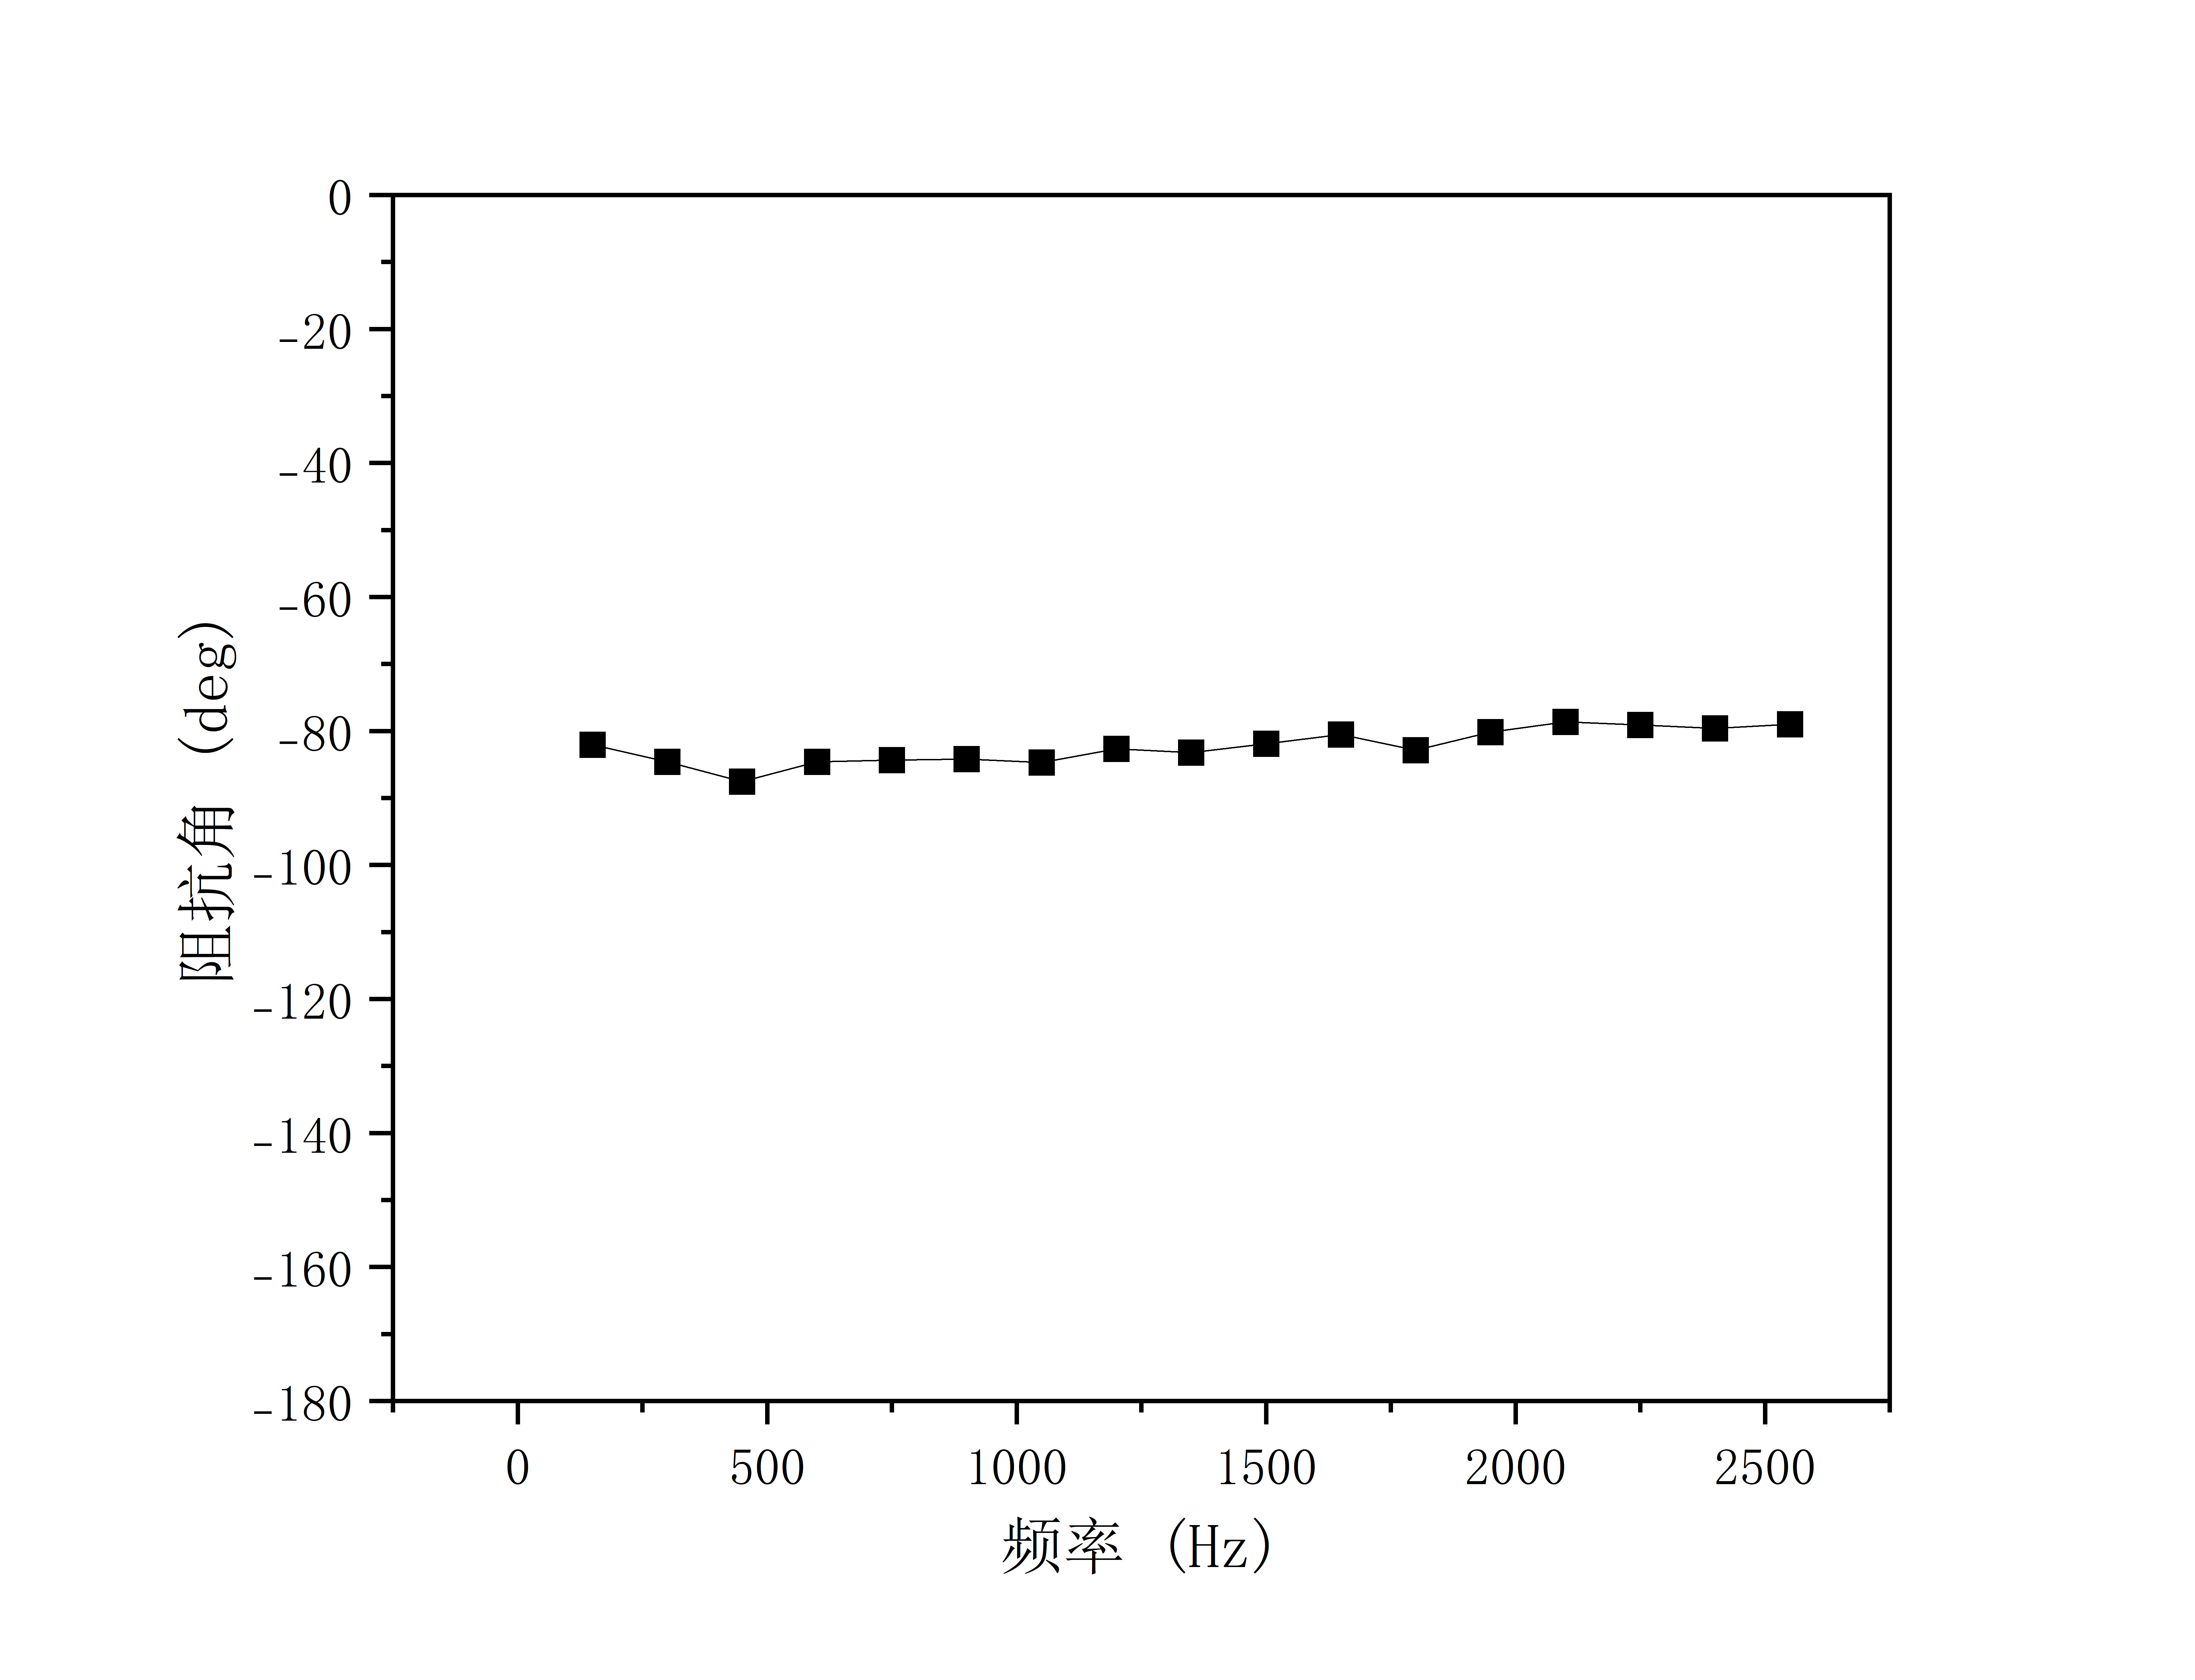
\includegraphics[width=0.7\textwidth]{4.png}}\\
            \caption{阻抗与频率关系曲线}
        \end{figure}\par
        实验中电感的阻抗角随频率变化的程度较大,感性显示出低频下不明显、高频下很明显的趋势,符合常规印象中电感“通低频,阻高频”的特性。拟合得到的 $k=\frac{L}{R}=1.71\text{E}-4$ 与图~\ref{fig:1} 得到的结果很接近(1.6E-4)。\par
        非理想的电容存在电阻参数和寄生参数,可以等效转化为理想电阻、电感、电容的串联。其复阻抗为:$Z=R+\mathrm{j}(2\pi f L-\dfrac{1}{2\pi f C})$。 在本次测量的频率范围内,因为频率相对于谐振频率过小,故表现出很明显的容性,阻抗角维持在 $-80^\circ$ 附近,有些许上升趋势;若频率进一步增加,可能会观察到阻抗角进一步增大,越过谐振点时阻抗角由负变为正值,随后进一步增大。
\section{思考题}
    \subsection{图 2 中各元件流过的电流如何求得?}
        电压有效值可以用示波器直接读取,电流则要根据采样电阻的电压使用欧姆定律求得。
    \subsection{怎样用双踪示波器观察 RL 串联和 RC 串联电路阻抗角的频率特性?}
        示波器分别测量 $U_\text{s}$ 和 $U_\text{r}$,同时使用示波器的运算功能得出 $U_\text{L}=U_\text{s}-U_\text{r}$ 的波形,这样就可以通过数格子或者自动测量功能测量出阻抗角。
\section{实验心得}
    本次实验探究了R、L、C 元件的阻抗特性,进一步讨论了实际电容、电感模型,通过拟合方法得到其参数,对 AC 电路又有了更加清晰明确的认知。
    \newpage
    \clearpage
\section{原始数据及图形}
    \begin{center}
        \begin{figure}[!ht]
            \subfloat[page1]{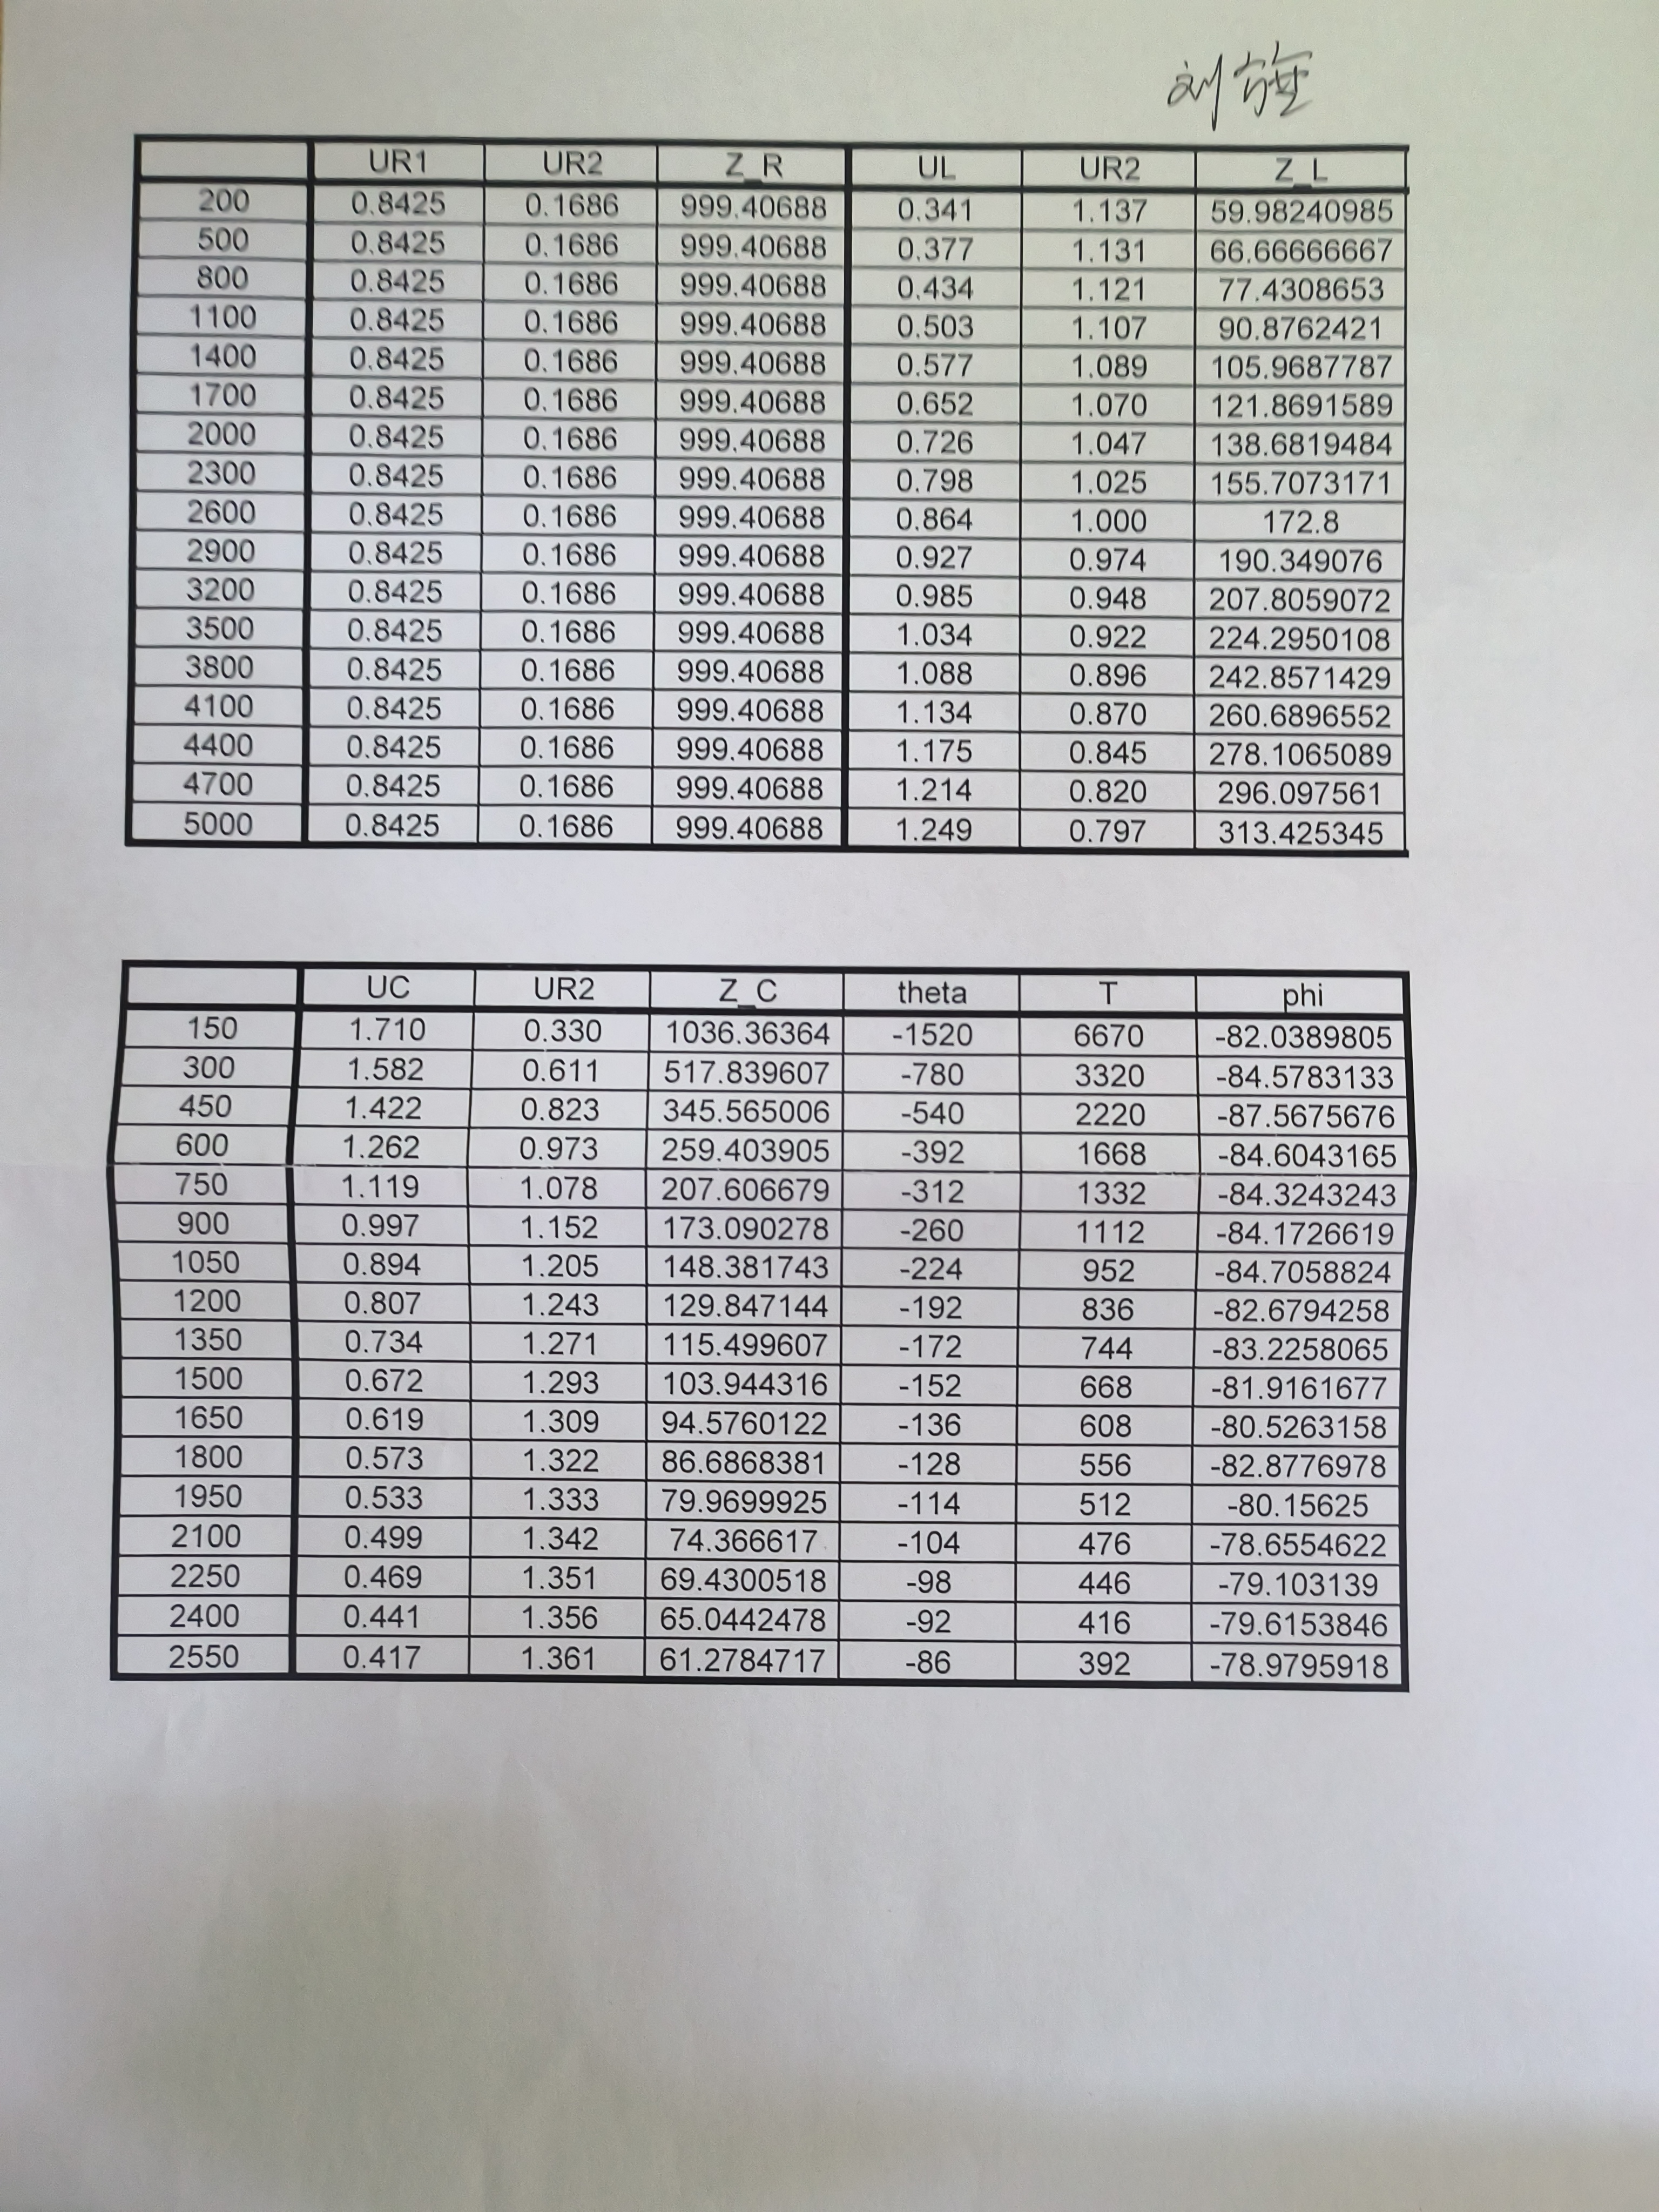
\includegraphics[width=0.43\textwidth]{5.jpg}}\hspace{6mm}
            \subfloat[page2]{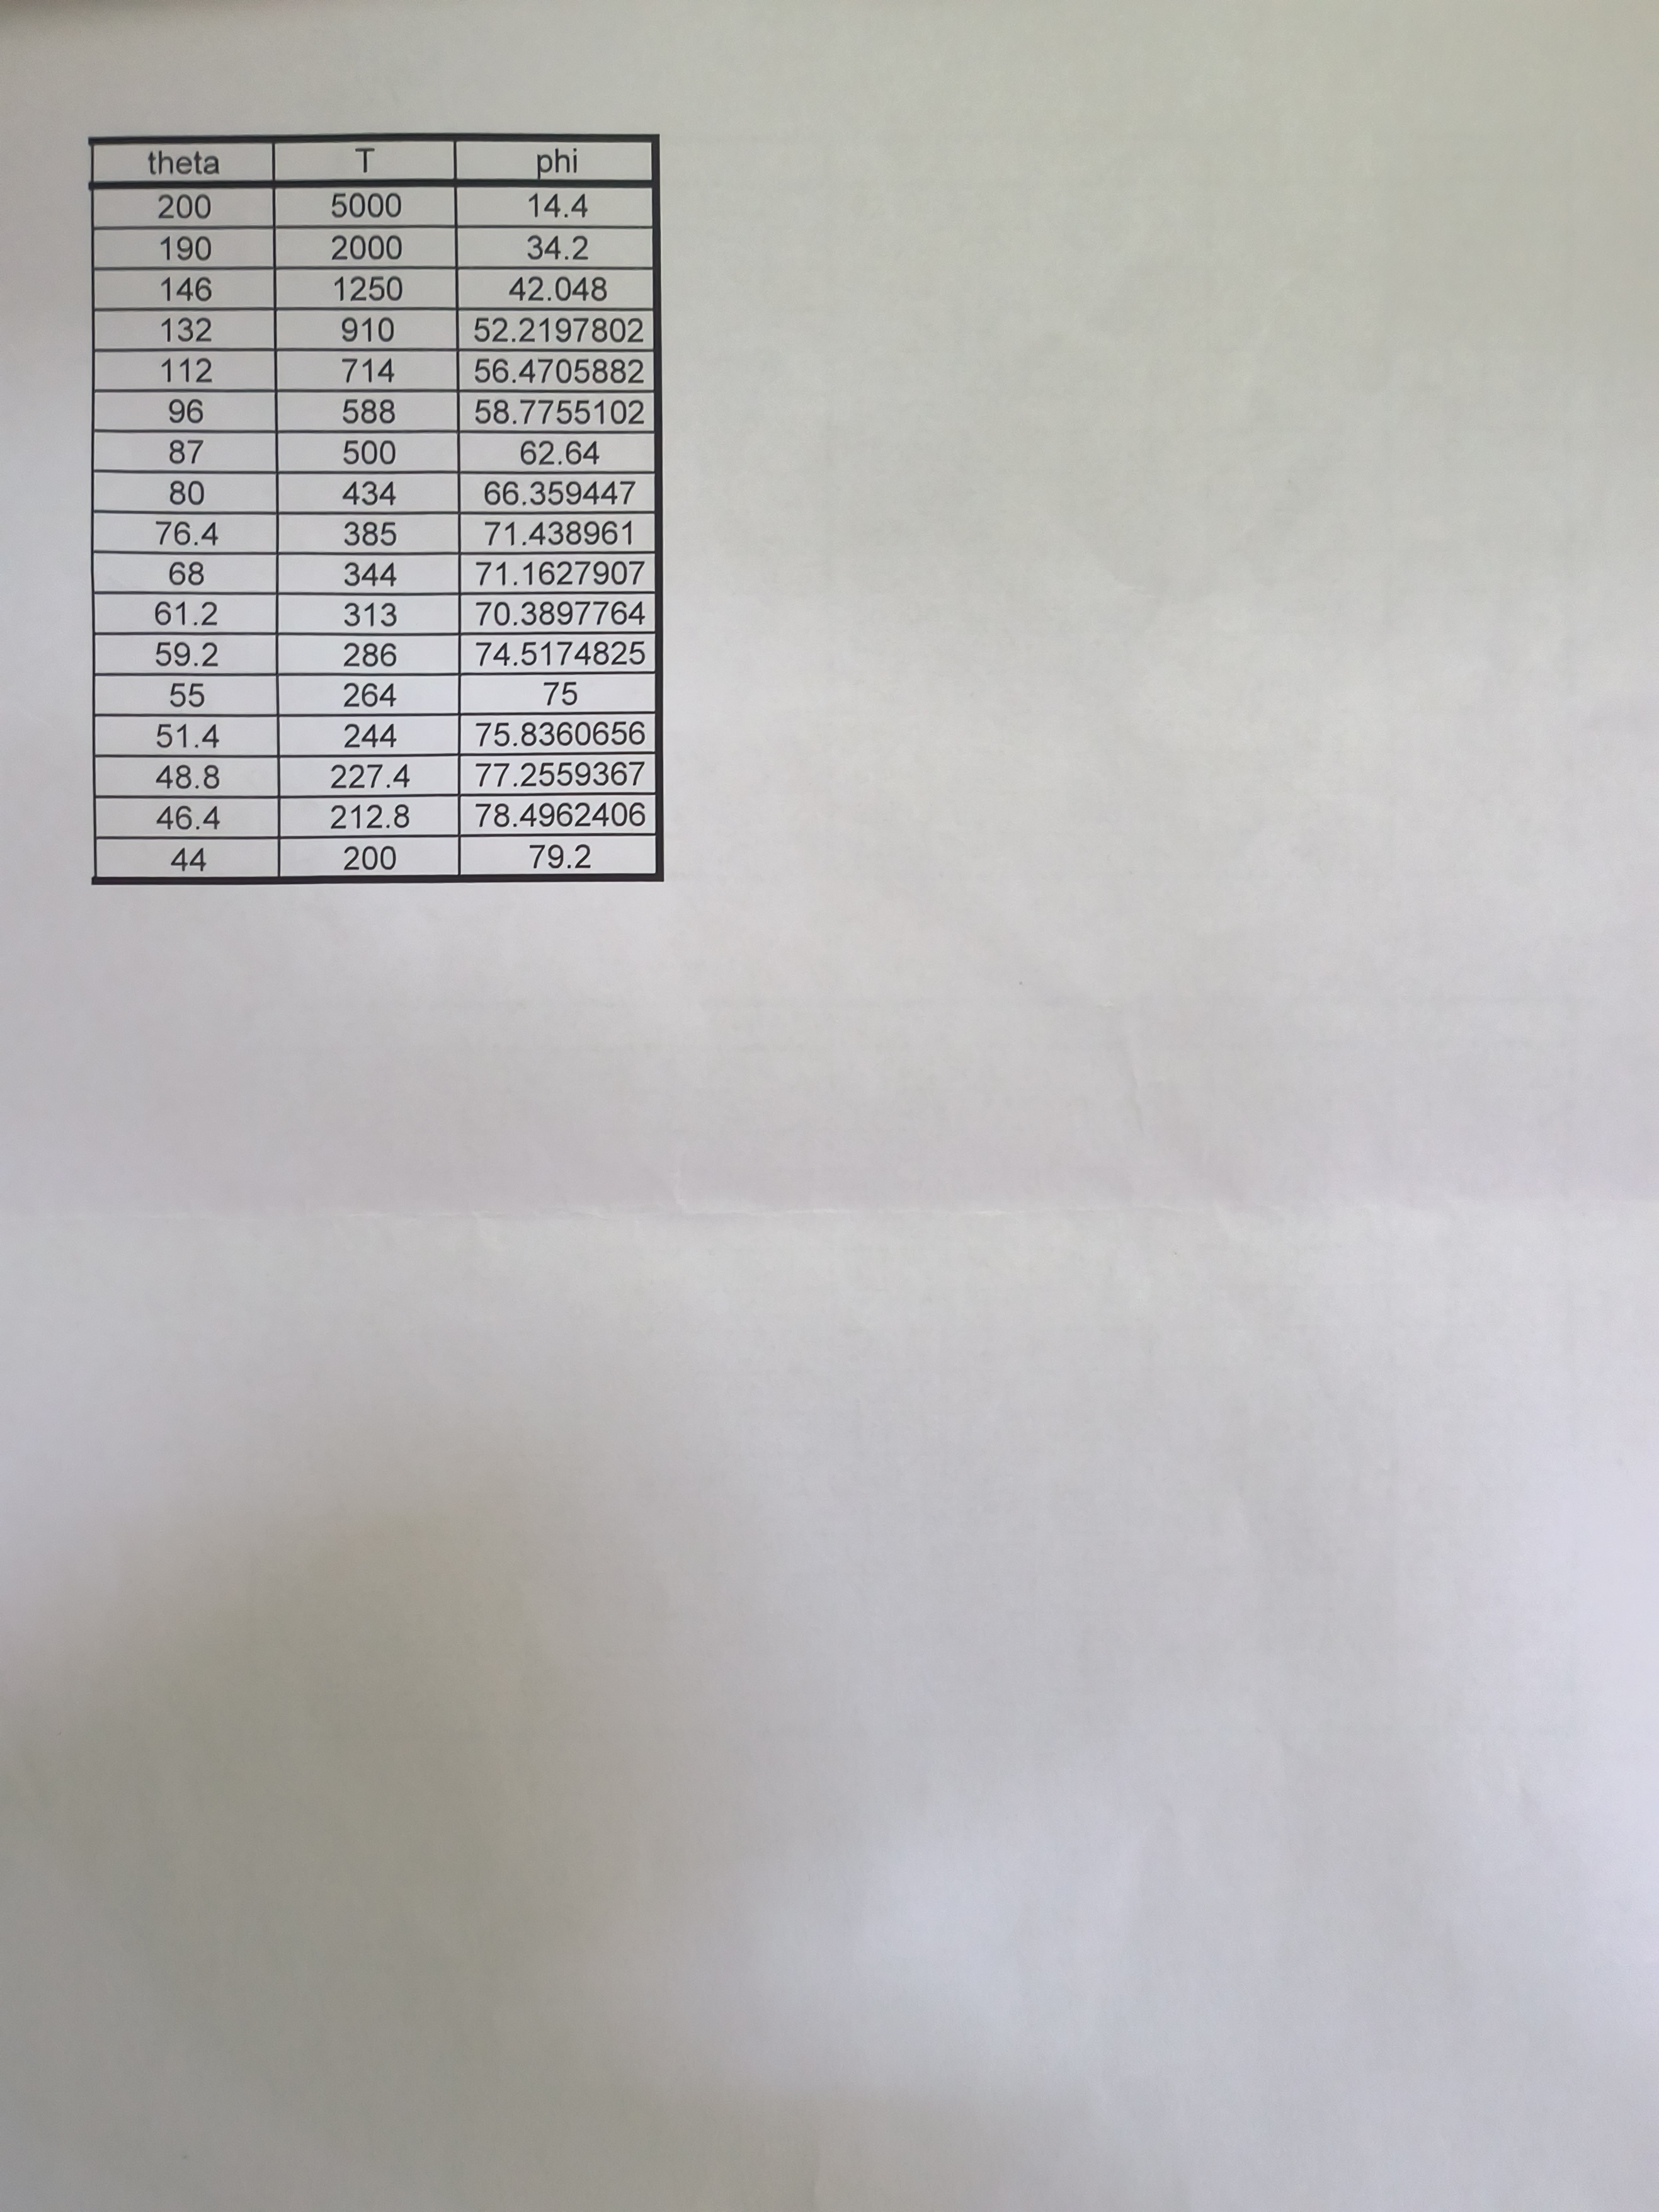
\includegraphics[width=0.43\textwidth]{6.jpg}}\\
        \end{figure}\par
    \end{center}
    \end{document}